\documentclass[12pt, a4paper, oneside, UTF8]{ctexart}
\usepackage{amsmath, amsthm, amssymb, bm, color, framed, graphicx, hyperref, mathrsfs}
\usepackage{geometry}
\usepackage{caption}
\geometry{left = 2.5 cm, right = 2.5 cm, top = 2.5 cm, bottom = 2.5 cm}

\title{\textbf{作业11}\\{\small (数值算法与案例分析)}}
\author{李维杰}
\date{\today}
\linespread{1.5}
\definecolor{shadecolor}{RGB}{241, 241, 255}
\newcounter{problemname}
\newenvironment{problem}{\begin{shaded}\stepcounter{problemname}\par\noindent\textbf{题目\arabic{problemname}. }}{\end{shaded}\par}
\newenvironment{solution}{\par\noindent\textbf{解答. }}{\par}
\newenvironment{note}{\par\noindent\textbf{注记. }}{\par}

\newcommand{\pll}{\kern 0.56em/\kern -0.8em /\kern 0.56em}

\begin{document}

\maketitle

\begin{problem}
    找一个使得Jacobi迭代收敛但Gauss-Seidel迭代不收敛的线性方程组,并证明.
\end{problem}

\begin{solution}
    设$$A=D - L - U = \left[
        \begin{array}{ccc}	
            1 & 2 & 1 \\
            -2 & 1 & -1 \\
            2 & -2 & 1
        \end{array}
    \right],$$
    则$\rho(D^{-1}(L+U)) = 0$,而$\rho((D-L)^{-1}U) = 2 + 2\sqrt{5}$,故对于该矩阵Jacobi迭代收敛但Gauss-Seidel迭代不收敛.
\end{solution}

\begin{problem}
    找一个使得Jacobi迭代不收敛但Gauss-Seidel迭代收敛的正定线性方程组,并证明.
\end{problem}

\begin{solution}
    设$$A=D - L - U = \left[
        \begin{array}{ccc}	
            2 & 1 & 1 \\
            -1 & 1 & 2 \\
            1 & 1 & 2
        \end{array}
    \right] \succ 0,$$
    则$\rho(D^{-1}(L+U)) = 1$,而$\rho((D-L)^{-1}U) = \frac{\sqrt{2}}{2}$,故对于该矩阵Jacobi迭代不收敛但Gauss-Seidel迭代收敛.
\end{solution}
\newpage
\begin{problem}
    设$B \in \mathbb{C}^{n \times n},g \in \mathbb{C}^{n}$, 并假定$\rho(B) = 0$.证明迭代方案$$x^{(k+1)}=Bx^{(k)}+g$$对于任意初始$x^{(0)}$都将在$n$步内收敛为$x=Bx+g$的解.
\end{problem}

\begin{solution}
    设残差$r^{(k)} = x^{(k)} - x$,则$$r^{(k+1)} = x^{(k+1)} - x = B x^{(k)} - Bx = B r^{(k)},$$
    故$r^{(n)} = B^n r^{(0)}$.结合$\rho(B) = 0$,可得$B^n = 0$,于是$$r^{(n)} = 0,$$即$x^{(n)}$收敛为$x$.
\end{solution}

\begin{problem}
    设$B,M \in \mathbb{C}^{n \times n},g \in \mathbb{C}^{n}$, 并假定$M$和$M-B^*MB$都是正定的.证明迭代方案$$x^{(k+1)}=Bx^{(k)}+g$$对于任意初始$x^{(0)}$都将收敛为$x=Bx+g$的解.
\end{problem}

\begin{solution}
    设$B$的任意特征对为$(\lambda, x)$,则$$x^*(M - B^*MB)x > 0 \Rightarrow x^* M x - (Bx)^* M (Bx) > 0 \Rightarrow (1-\lambda^2)x^* M x > 0.$$
    结合$x^* M x > 0$,可得$\lambda^2 < 1$,也即$$\rho(B) < 1.$$于是对于任意初始$x^{(0)}$,该收敛方案均能收敛.
\end{solution}

\begin{problem}
    在数值意义上解单位正方形$[0,1]^2$上的2D拉普拉斯方程$$\frac{\partial^2 u}{\partial x^2} + \frac{\partial^2 u}{\partial y^2} = 0.$$
    该方程有边界条件$$u(0,y)=u(1,y)=u(x,1)=0,y(x,0)=\sin(\pi x).$$
    使用Jacobi迭代或Gauss-Seidel迭代来解这个离散系统.可视化解和收敛历程.
\end{problem}
    
\begin{solution}
    (代码见Problem5.m)
    \begin{figure}[h]
        \centering
        \begin{minipage}[b]{0.3\textwidth}
            \centering
            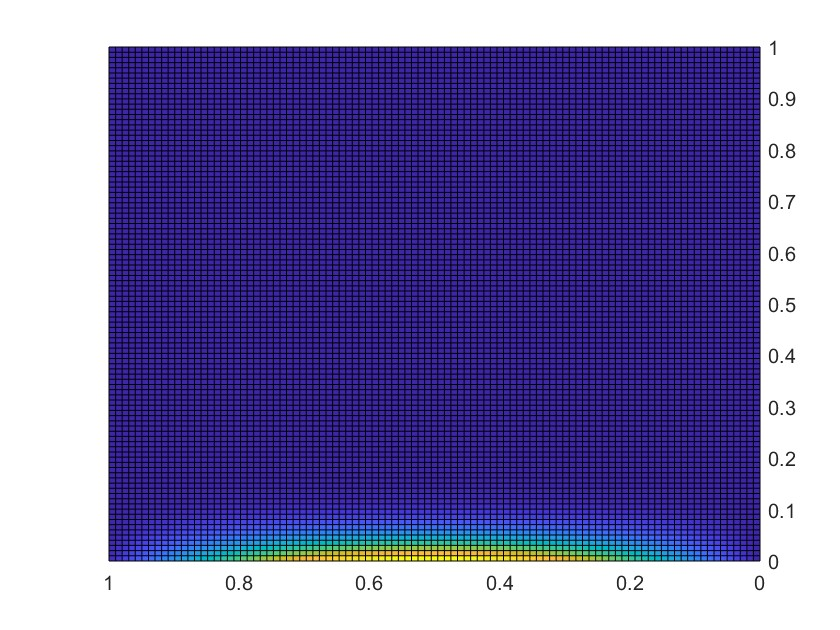
\includegraphics[width=\textwidth]{Jacobi_1.jpg}
            \caption{iter=0}
        \end{minipage}
        \begin{minipage}[b]{0.3\textwidth}
            \centering
            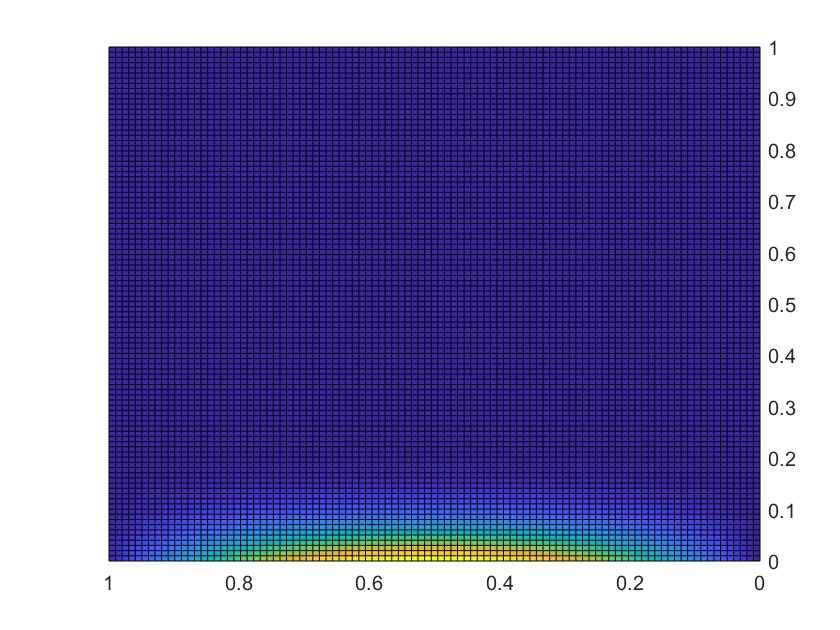
\includegraphics[width=\textwidth]{Jacobi_2.jpg}
            \caption{iter=50}
        \end{minipage}
        \begin{minipage}[b]{0.3\textwidth}
            \centering
            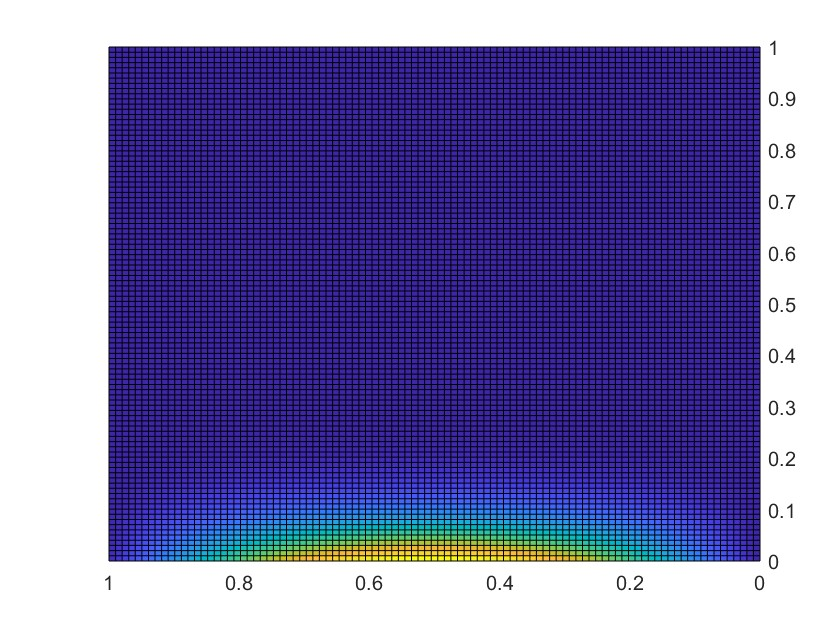
\includegraphics[width=\textwidth]{Jacobi_3.jpg}
            \caption{iter=100}
        \end{minipage}
    \end{figure}
    
    \begin{figure}[h]
        \centering
        \begin{minipage}[b]{0.3\textwidth}
            \centering
            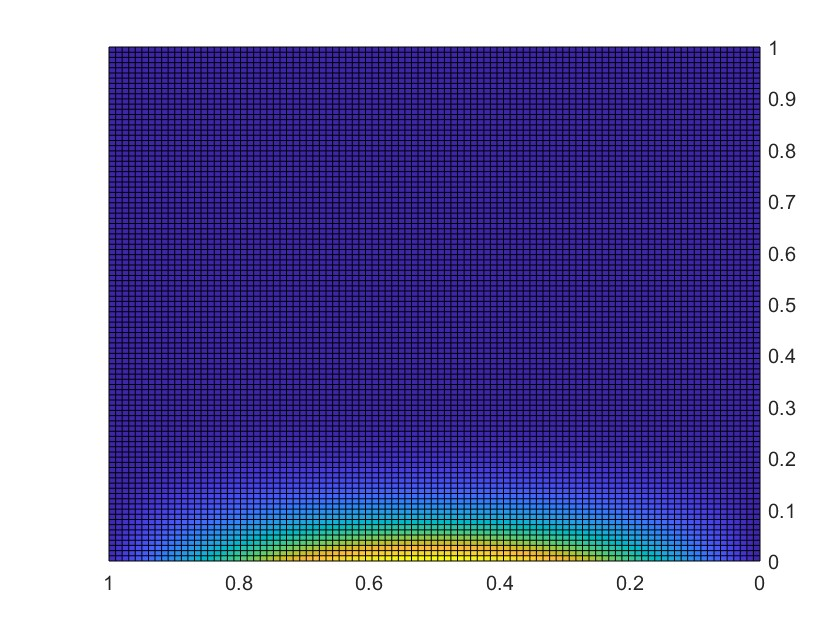
\includegraphics[width=\textwidth]{Jacobi_4.jpg}
            \caption{iter=150}
        \end{minipage}
        \begin{minipage}[b]{0.3\textwidth}
            \centering
            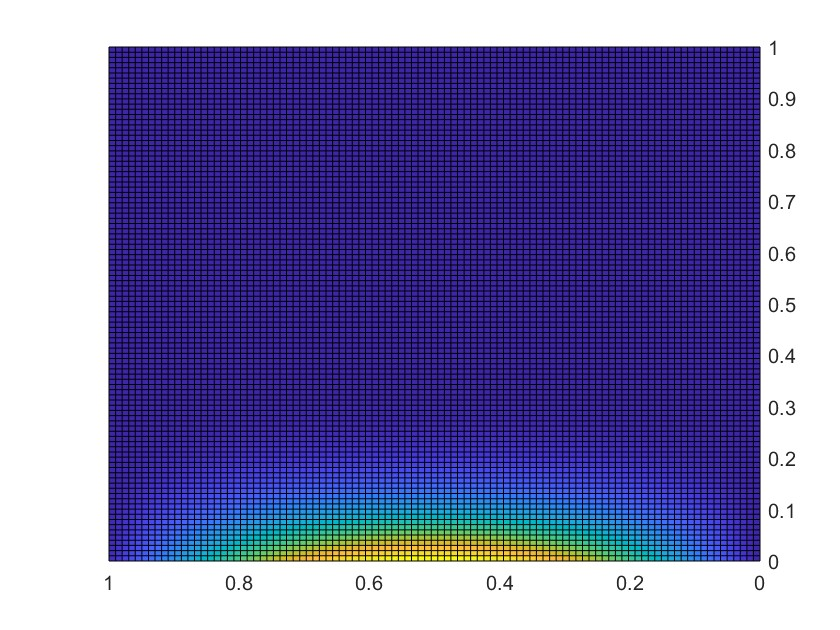
\includegraphics[width=\textwidth]{Jacobi_5.jpg}
            \caption{iter=200}
        \end{minipage}
        \begin{minipage}[b]{0.3\textwidth}
            \centering
            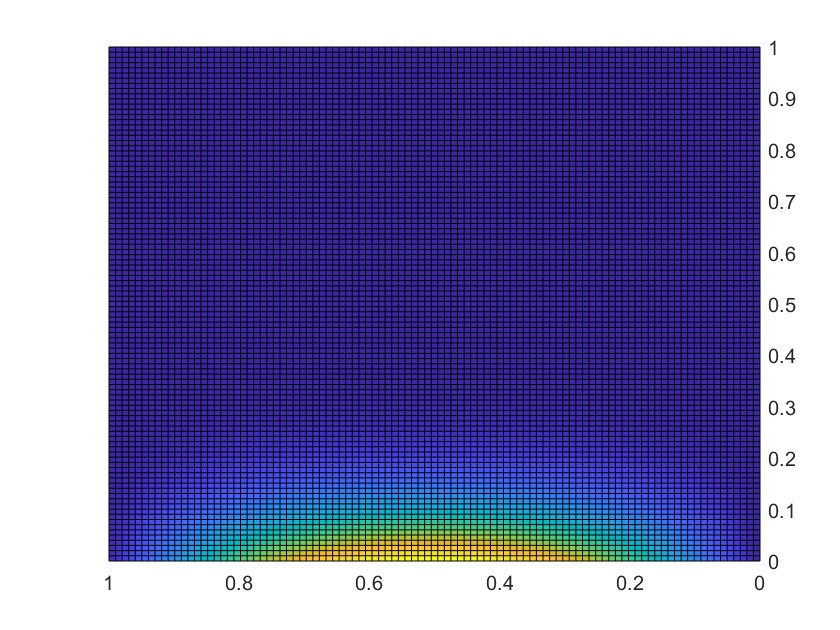
\includegraphics[width=\textwidth]{Jacobi_6.jpg}
            \caption{iter=250}
        \end{minipage}
        \captionsetup{labelformat=empty}  % 禁用编号
        \caption{Jacobi迭代(初始设定$u=0$)}  % 只显示标题,没有编号
    \end{figure}
    \begin{figure}[htbp]
        \centering
        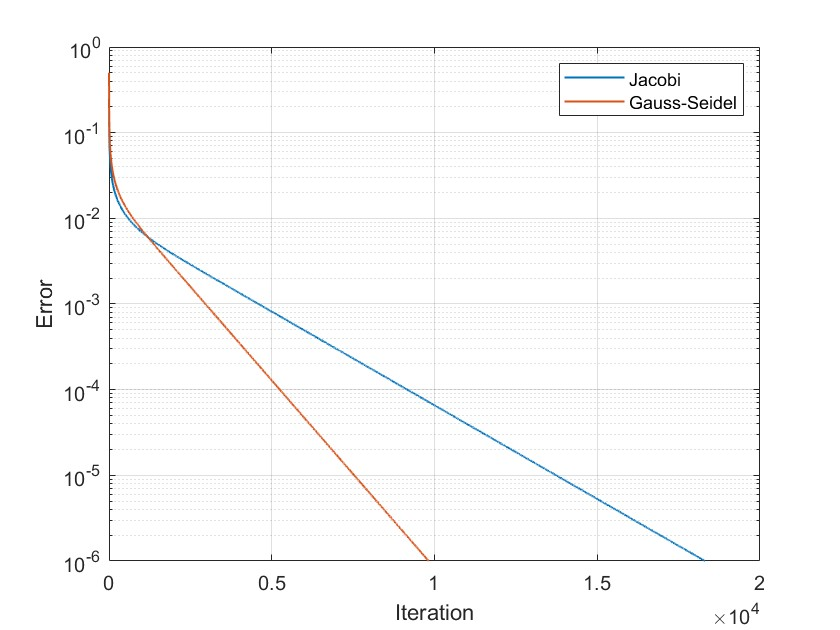
\includegraphics[scale=0.5]{Convergence_History.jpg}
        \captionsetup{labelformat=empty}
        \caption{Jacobi迭代和Gauss-Seidel迭代的收敛历程}
    \end{figure}
\end{solution}

\end{document}